 %% Simplified vision for Ausarbeitungen
\documentclass[%
paper=a4,      % alle weiteren Papierformat einstellbar
fontsize=11pt, % Schriftgr��e (12pt, 11pt (Standard))
BCOR1cm,       % Bindekorrektur, bspw. 1 cm
DIV15,         % f�hrt die Satzspiegelberechnung neu aus s. scrguide 2.4
%twoside,       % Doppelseiten
headsepline,   %
headings=openright, % Kapitel nur rechts beginnen
%biblography=totoc, % Literaturverzeichnis einf�gen bibtotocnumbered: nummeriert
parskip=half,  % Europ�ischer Satz mit Abstand zwischen Abs�tzen
chapterprefix, % Kapitel anschreiben als Kapitel
headsepline,   % Linie nach Kopfzeile
titlepage,     %
numbers=noenddot,
%draft	       % zeigt �berlange Zeilen an
]{scrreprt}

\usepackage{pdfpages}       % Titelseite hat ein anderes Layout. Sie wird 
                            % separat erzeugt und hier eingef�gt
\usepackage[T1]{fontenc}
\usepackage[utf8]{inputenc}  % Zeichencodierung
\usepackage[ngerman, english]{babel} % Worttrennung nach neuer Rechtschreibung
%\usepackage[ngerman]{babel}
\usepackage{siunitx}
\usepackage{ellipsis}       % Leerraum um Auslassungspunkte
\usepackage{fixltx2e}       % Fehlerkorrektur Zeichens�tze
\usepackage{xspace}         % f�ge evtl. notwendiges Leerzeichen hinzu (\xspace)
\usepackage{textcomp}
\usepackage{bm}
\usepackage{enumerate}


%\usepackage{mathptmx}           % Times + passende Mathefonts
\usepackage{mathpazo}           % Palatino + passende Mathefonts
\usepackage[scaled=.92]{helvet} % skalierte Helvetica als \sfdefault
\usepackage{courier}            % Courier als \ttdefault

\usepackage{graphicx}    % Einbindung von Grafiken
\graphicspath{{Images/}} % Unterverzeichnis, in dem Grafiken abgelegt werden
\usepackage{listings}    % Listenausgabe externer Dateien
\lstset{language=Matlab}
% \usepackage[framed,numbered,autolinebreaks,useliterate]{mcode}

\usepackage{float}      % Paket zum Erweitern der Floatumgebungen
\usepackage[figuresright]{rotating}   % Rotieren von Objekten
%\usepackage{hvfloat}
\usepackage{array}      % Paket zum Erweitern der Tabelleneigenschaften
\usepackage{booktabs}   % Paket f�r sch�nere Tabellen

\usepackage{amsmath}    % erweiterte Mathematik-Umgebungen
\usepackage{amssymb}
\usepackage{url}



% Einstellungen f�r das Literaturverzeichnis
\usepackage[round]{natbib}
\setlength{\bibsep}{0.5\baselineskip}
\setlength{\bibhang}{1cm}
\bibliographystyle{agsm}

% Andere Schriftarten in Koma-Script
\setkomafont{sectioning}{\normalfont\bfseries}
\setkomafont{captionlabel}{\rmfamily\bfseries\small}
\setkomafont{caption}{\mdseries\itshape\small}
\setkomafont{pagehead}{\normalfont\itshape} % Kopfzeilenschrift
\setkomafont{descriptionlabel}{\normalfont\bfseries}

% Kopf und Fu�zeilen
\usepackage[automark]{scrlayer-scrpage}

% Hyperref
\usepackage{hyperref}

% Literaturverzeichnis-Stil
\bibliographystyle{plain}

% weitere Einstellungen
\tolerance=200               % �bervolle Zeile vermeiden
\emergencystretch=3em

\clubpenalty=10000           % 'Schusterjungen' und 'Hurenkinder' vermeiden
\widowpenalty=10000 
\displaywidowpenalty=10000

\parindent 0pt               % Einzug zu Absatzbeginn festlegen

\setcapindent{1em}           % Zeilenumbruch bei Bildbeschreibungen.

\setcounter{secnumdepth}{3}  % Strukturiertiefe bis subsubsection{} m�glich
\setcounter{tocdepth}{3}     % Dargestellte Strukturiertiefe im Inhaltsverzeichnis

% Korrekturversion mit 1.5-fachem Zeilenabstand im Hauptteil:
\newif\ifiscorrect
%\iscorrecttrue   % Korrekturversion
\iscorrectfalse % keine Korrekturversion

%% Eigene Definitionen:

% Einheiten:
\def\ut#1{\ensuremath{\,\mathrm{#1}}}

% Operatoren:
\def\grad{\ensuremath{\mathop{\mathrm{grad}}\nolimits}}
\def\transp#1{\ensuremath{{#1}^\mathsf{T}}}  % transpose
\def\const{\ensuremath{\mathop{\mathrm{const.}}\nolimits}}

% Formelzeichen:
\def\vec#1{\ensuremath{\mathbf{#1}}}
\def\matr#1{\ensuremath{\mathbf{#1}}}

% Hack, um ein zus�tzliches Leerzeichen nach \input zu entfernen:
\def\myinput#1{%
  \endlinechar=-1 % kein Zeilenabschlusszeichen
  \input #1\relax
  \endlinechar `\^^M % Zeilenabschluss = Zeilenvorschub
}



\begin{document}
\selectlanguage{ngerman}
\pagenumbering{Roman}
\pagestyle{plain}

%% Title

\includepdf[pages=1]{title}

%% Table of contents
\pagestyle{scrheadings}
\clearscrheadfoot            % Standardkram wegwerfen
\ohead[\pagemark]{\pagemark} % oben au�en Seitenzahl 
%% Ausarbeitung简化版目录,只保留内容目录
\tableofcontents
\clearpage

% Pages number: roemisch
% Nmber in the text: arabic
\newcounter{roemisch}
\setcounter{roemisch}{\value{page}}
\pagenumbering{arabic}

\ifiscorrect\linespread{1.5}\selectfont % ???: 1 1/2 (f�r bessere Korrektur)
\else\fi

%% Chapters
% Kopfzeile: links Kapitel, rechts Sektion
\clearscrheadfoot            % Standardkram wegwerfen
\ohead[\pagemark]{\pagemark} % oben au�en Seitenzahl 
\ihead{\headmark}            % oben innen automatischer Abschnittsname
\automark[]{section}
\chapter*{Ausarbeitung}

\section{Gezeitenpotential}

Gegeben sei der Punkt $P$ mit den sphärischen Koordinaten ($\lambda = 8.33^{\circ},~ \varphi = 48.14^{\circ},~r = 6366837~m$). Im Folgenden wird berechnet: 

\begin{enumerate}[a)]
\item Berechnung der Zeitreihe der Koeffizienten $v_{2,m}^{tid}$ 

Die Zeitreihe der Koeffizienten $v_{2,m}^{tid}$ vom Grad 2 des vom Mond erzeugten Gezeitenpotentials werden nun berechnet. Dabei werden explizit die Werte vom 15. Januar angegeben. Um die Zeitreihe zu berechnen wird folgende Formel herangezogen: 

\begin{gather*}
V^{tid}(\lambda, \phi, r) = \sum_{l=2}^{L} \sum_{m=-l}^{l} \left(\dfrac{r}{R}\right)^l v_{l,m}^{tid} \overline{Y}_{l,m}(\lambda,\phi) \\
v_{l,m}^{tid} = \dfrac{GM_{Moon}}{r_{Moon}} \dfrac{1}{2l+1} \left(\dfrac{R}{r_{Moon}}\right)^l \overline{Y}_{l,m} (\lambda_{Moon},\phi_{Moon}) \\
= \begin{bmatrix}
-0.5885 &  0.4409 &  -0.8039  & -0.0927 & -1.3381
\end{bmatrix}
\end{gather*} 

\item Berechnung des Gezeitenpotentials $v_{tid}$ 

Hier wird das vom Mond erzeugte Gezeitenpotential $v_{tid}$ berechnet. Anschließend werden die Zahlenwerte für den 1. bis 5. Januar angegeben. 

\begin{gather*}
v_{tid} = \begin{bmatrix}
-1.4564&-1.3540&-1.2456&-1.1379&-1.0388
\end{bmatrix}
\end{gather*}

\begin{figure}[H]
\centering
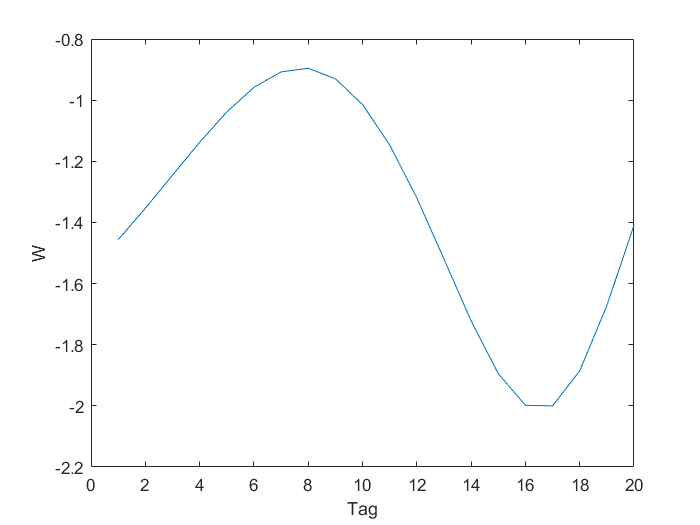
\includegraphics[scale=0.6]{gezpot.png}
\caption{Gezeitenpotential im Berechnungspunkt}
\label{gezpot}
\end{figure}

Abbildung \ref{gezpot} zeigt das Gezeitenpotential im Berechnungspunkt für das gesamte Zeitintervall im Januar. 

\item Berechnung des Gezeitenvektors $g_{tid}$

Nun wird der zugehörige Gezeitenvektor $g_{tid}$ für den 20. Januar berechnet. Dabei wird das ganze auf Terme vom Grad 2 beschränkt. 

\begin{gather*}
g_{tid} = \begin{bmatrix}
-0.4434 &-0.1148 &-0.9148
\end{bmatrix}
\end{gather*}
\end{enumerate}

\section{Gezeitenkatalog HW95}

Aus dem Gezeitenkatalog HW95, welches 12935 Partialtiden der Sonne, des Mondes und einiger Planeten enthält, soll das vom Mond erzeugte Gezeitenpotential $v_{tid}$, sowie der zugehörige Gezeitenvektor $g_{tid}$ für denselben Beobachtunspunkt und dieselben Zeitpunkte wie in Aufgabe 1 berechnet werden. 




\ifiscorrect\linespread{1.0}\selectfont% Zeilenabstand wieder auf 1 zur�ck
\else\fi

% Setze Numerierung wieder auf r�misch zur�ck und setzte von oben fort
% Wert ist demnach der von 'roemisch'
\newpage
\pagenumbering{Roman}
\setcounter{page}{\value{roemisch}}


\end{document}
